\chapter{Poorly measured lepton \ad at large $|\eta|$}
\label{large_eta}

We require muons to have $|\eta|<1.5$ due to the observed increase in width of the muon $d_0$ distribution at large $|\eta|$ in DY simulation with\ztautaull events removed (see Fig.~\ref{large_eta_mu} (left)). The width visibly increases at large $|\eta|$ in all three years but is less pronounced in 2017 and 2018 due to the improved performance of the Phase 1 pixel detector. The upgraded pixel detector is also responsible for the overall difference in $d_0$ width between years. Requiring muon $|\eta|< 1.5$ has two effects: (1) it dramatically reduces the mismeasurement background in 2016 data in the $\Pgm\Pgm$ channel, and (2) it removes a possible source of \ada-\adb correlation in which the correlation between muons in $\eta$ leads to correlation between muons in \ad. As shown in Fig.~\ref{large_eta_mu} (right), muons from \stoptolb events tend to have small $|\eta|$, so requiring muon $|\eta|< 1.5$ has a minimal effect on the signal acceptance.

\begin{figure}
\centering
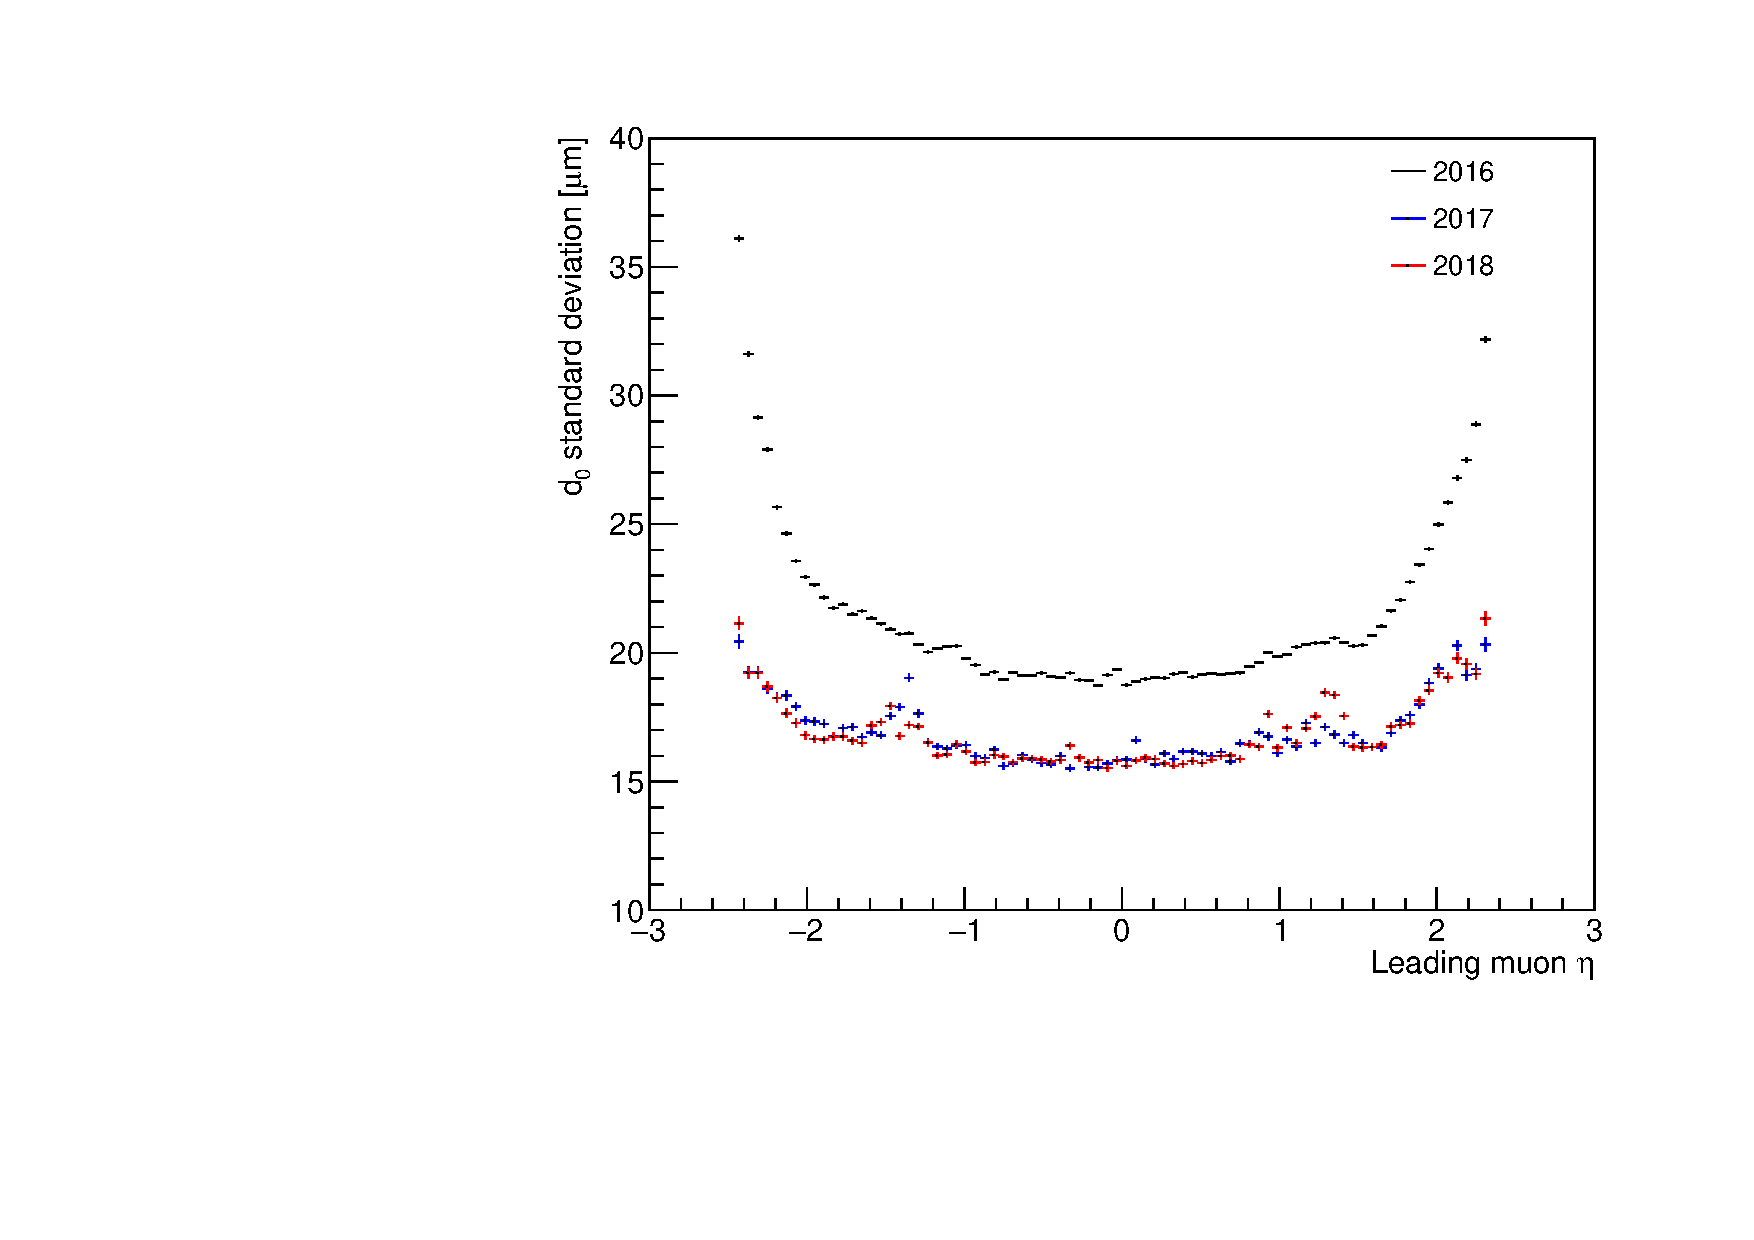
\includegraphics[width=0.5\textwidth]{figures/large_eta/d0_stdDev_vs_eta_compareYears.pdf}
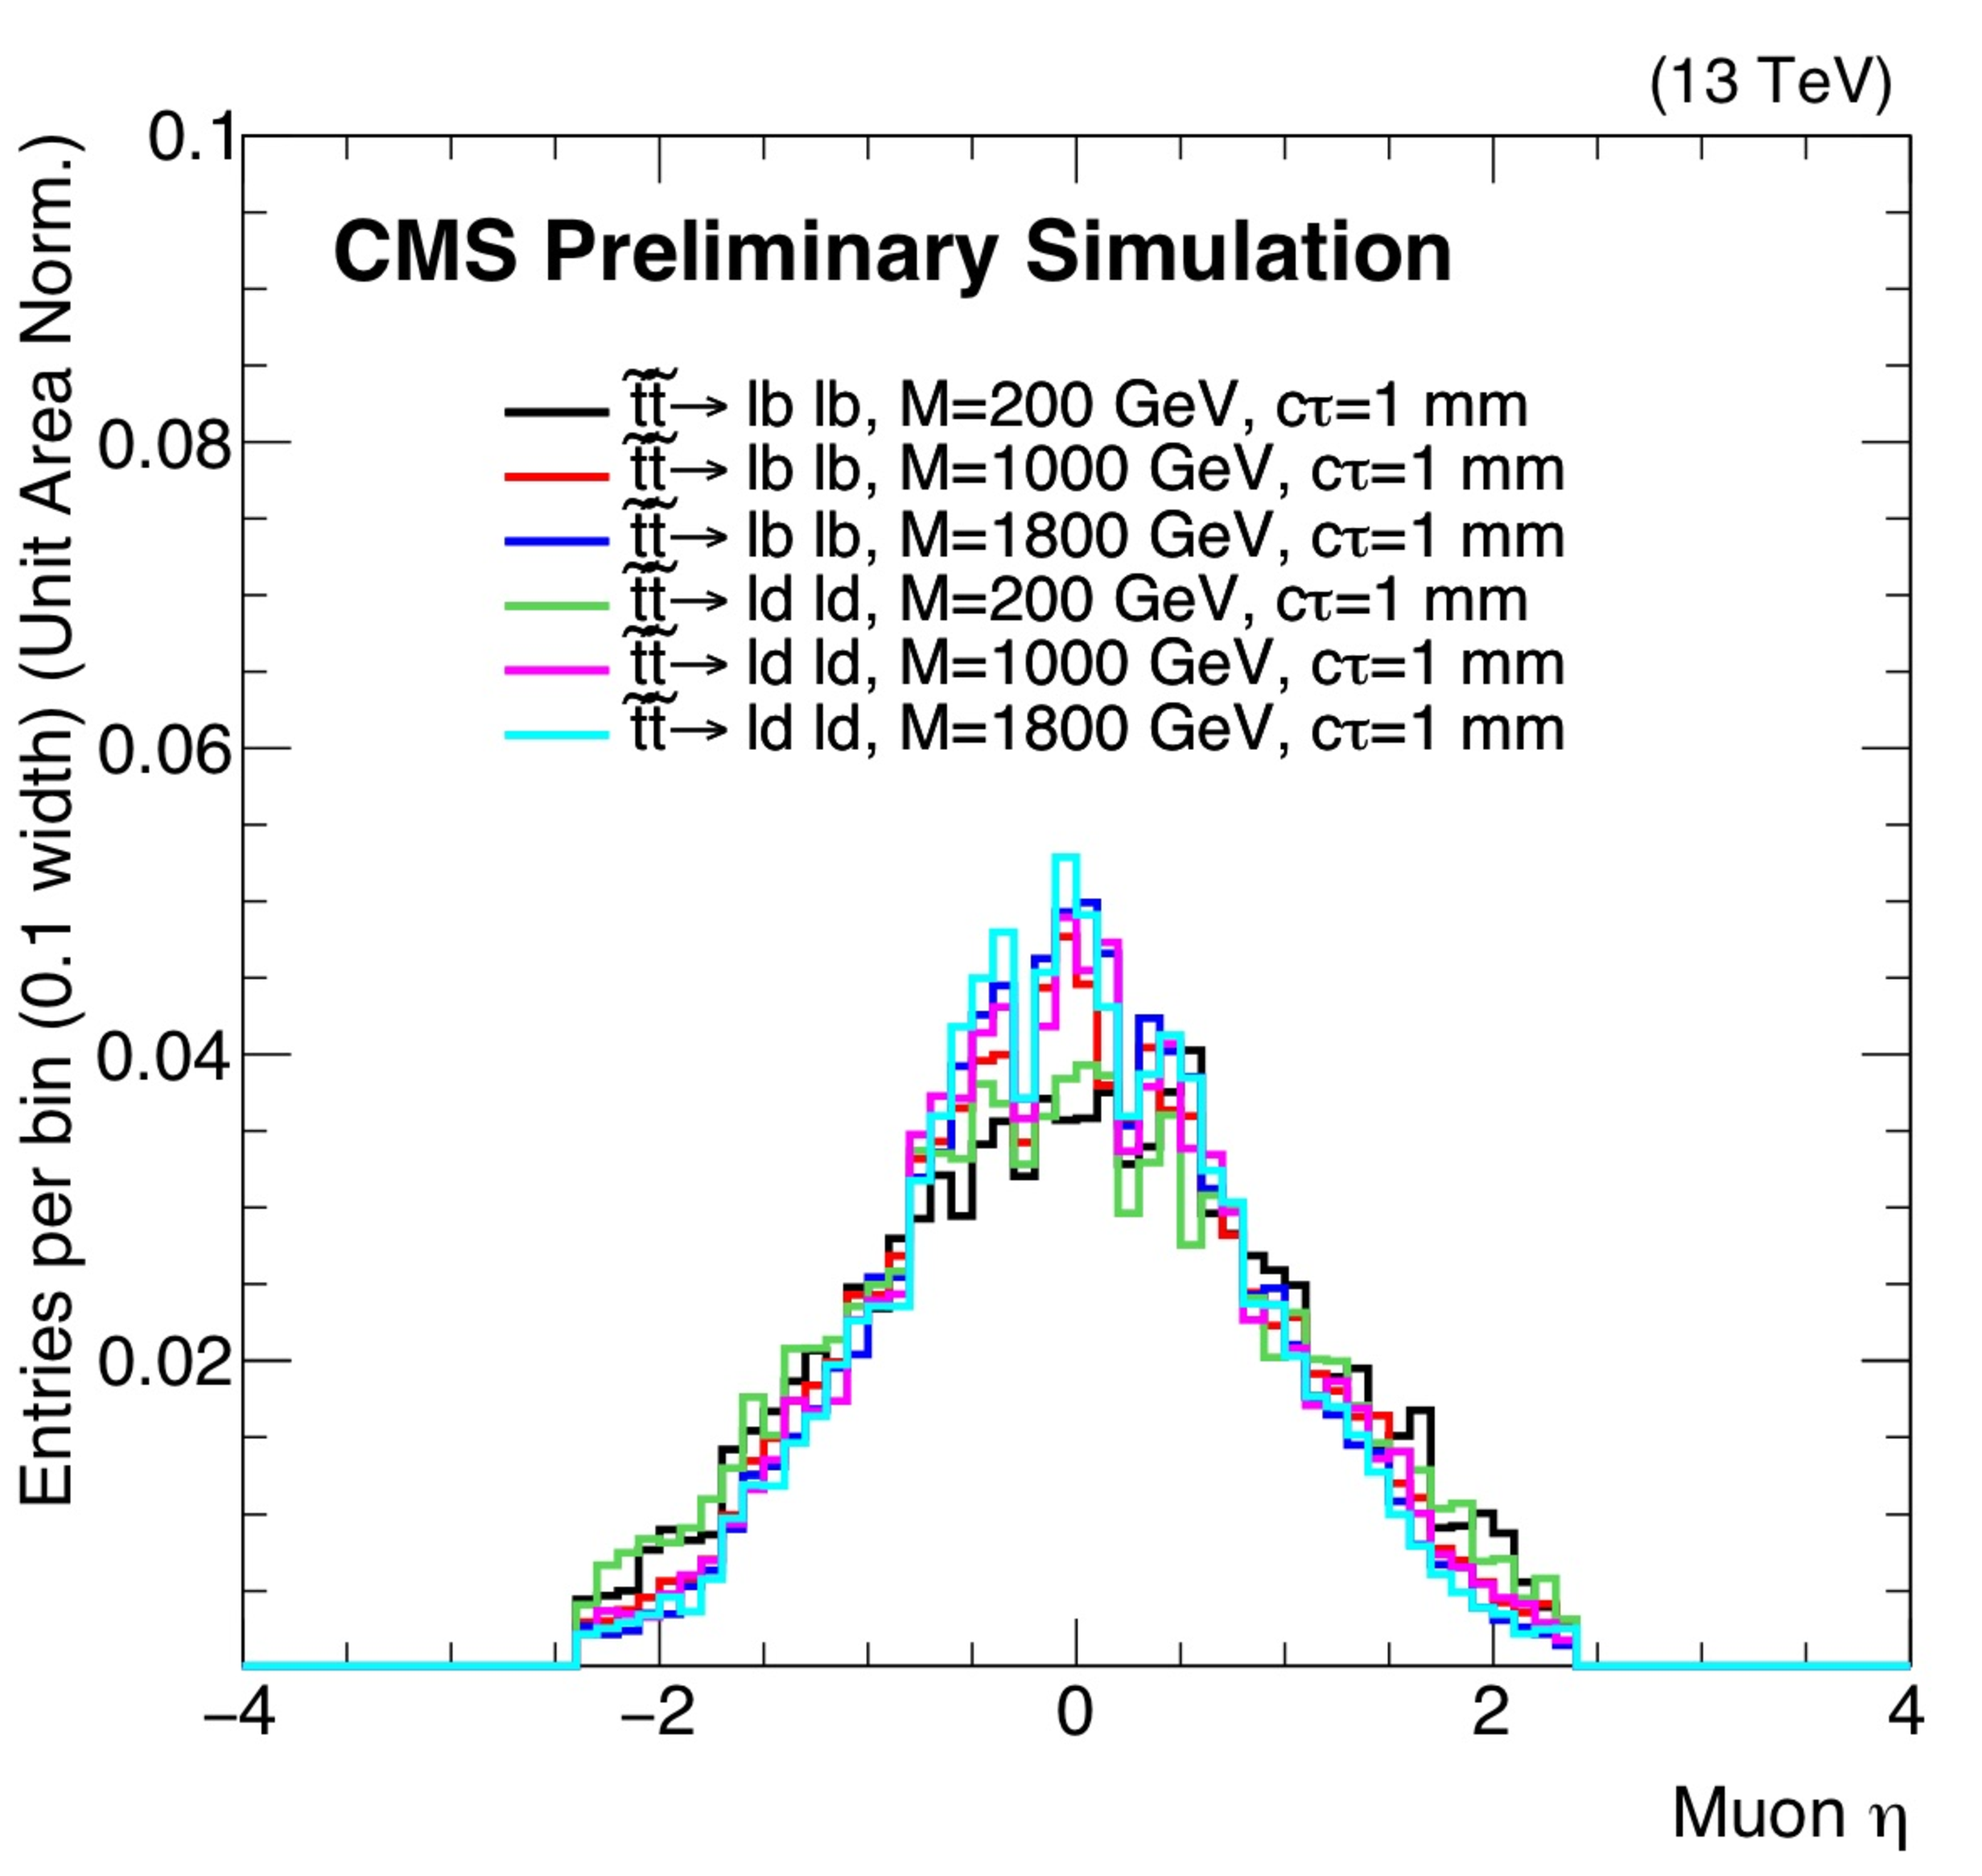
\includegraphics[width=0.43\textwidth]{figures/large_eta/muonEta.pdf}
\caption{The standard deviation of the leading muon $d_0$ as a function of the leading muon $\eta$ for simulated background events (left). To ensure that the variation in width is purely due to $d_0$ resolution effects, we use a sample of simulated Drell-Yan events from which the \ztautaull events have been removed. Muon $\eta$ distribution for simulated \stoptolb events (right). The $\Pgm\Pgm$ preselection with a loosened $|\eta|$ requirement is applied in both plots.}
\label{large_eta_mu}
\end{figure}

Electron $d_0$ resolution also worsens at large $|\eta|$. Furthermore, Fig.~\ref{large_eta_e} (left) shows that electrons from SM mesons are particularly concentrated $|\eta|>1.5$. As in the muon case, electrons from \stoptolb events tend to have $|\eta|<1.5$ (see Fig.~\ref{large_eta_e}), which implies that requiring electron $|\eta|<1.5$ will reduce the mismeasurement and SM meson backgrounds without significantly reducing signal acceptance.

\begin{figure}
\centering
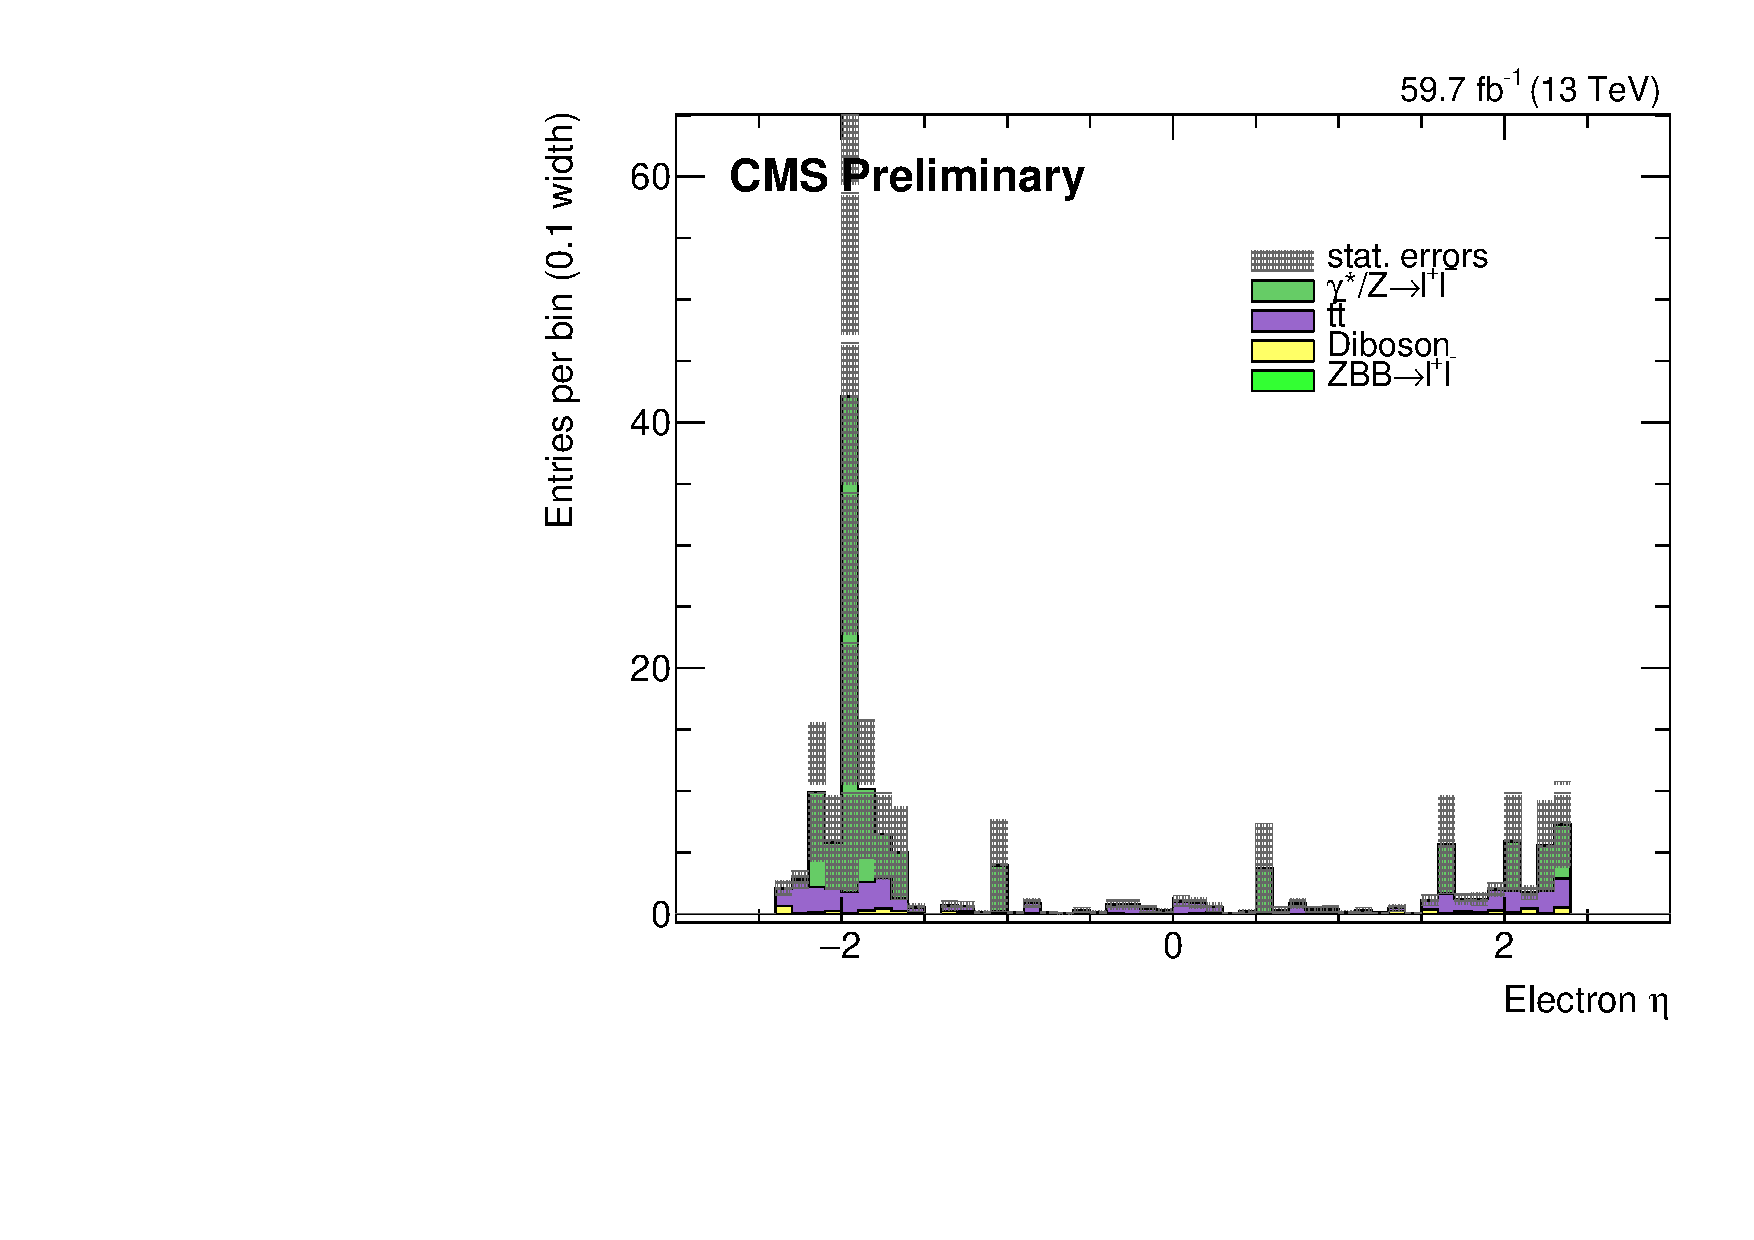
\includegraphics[width=0.5\textwidth]{figures/large_eta/electronEtaBkgLightMesons.pdf}
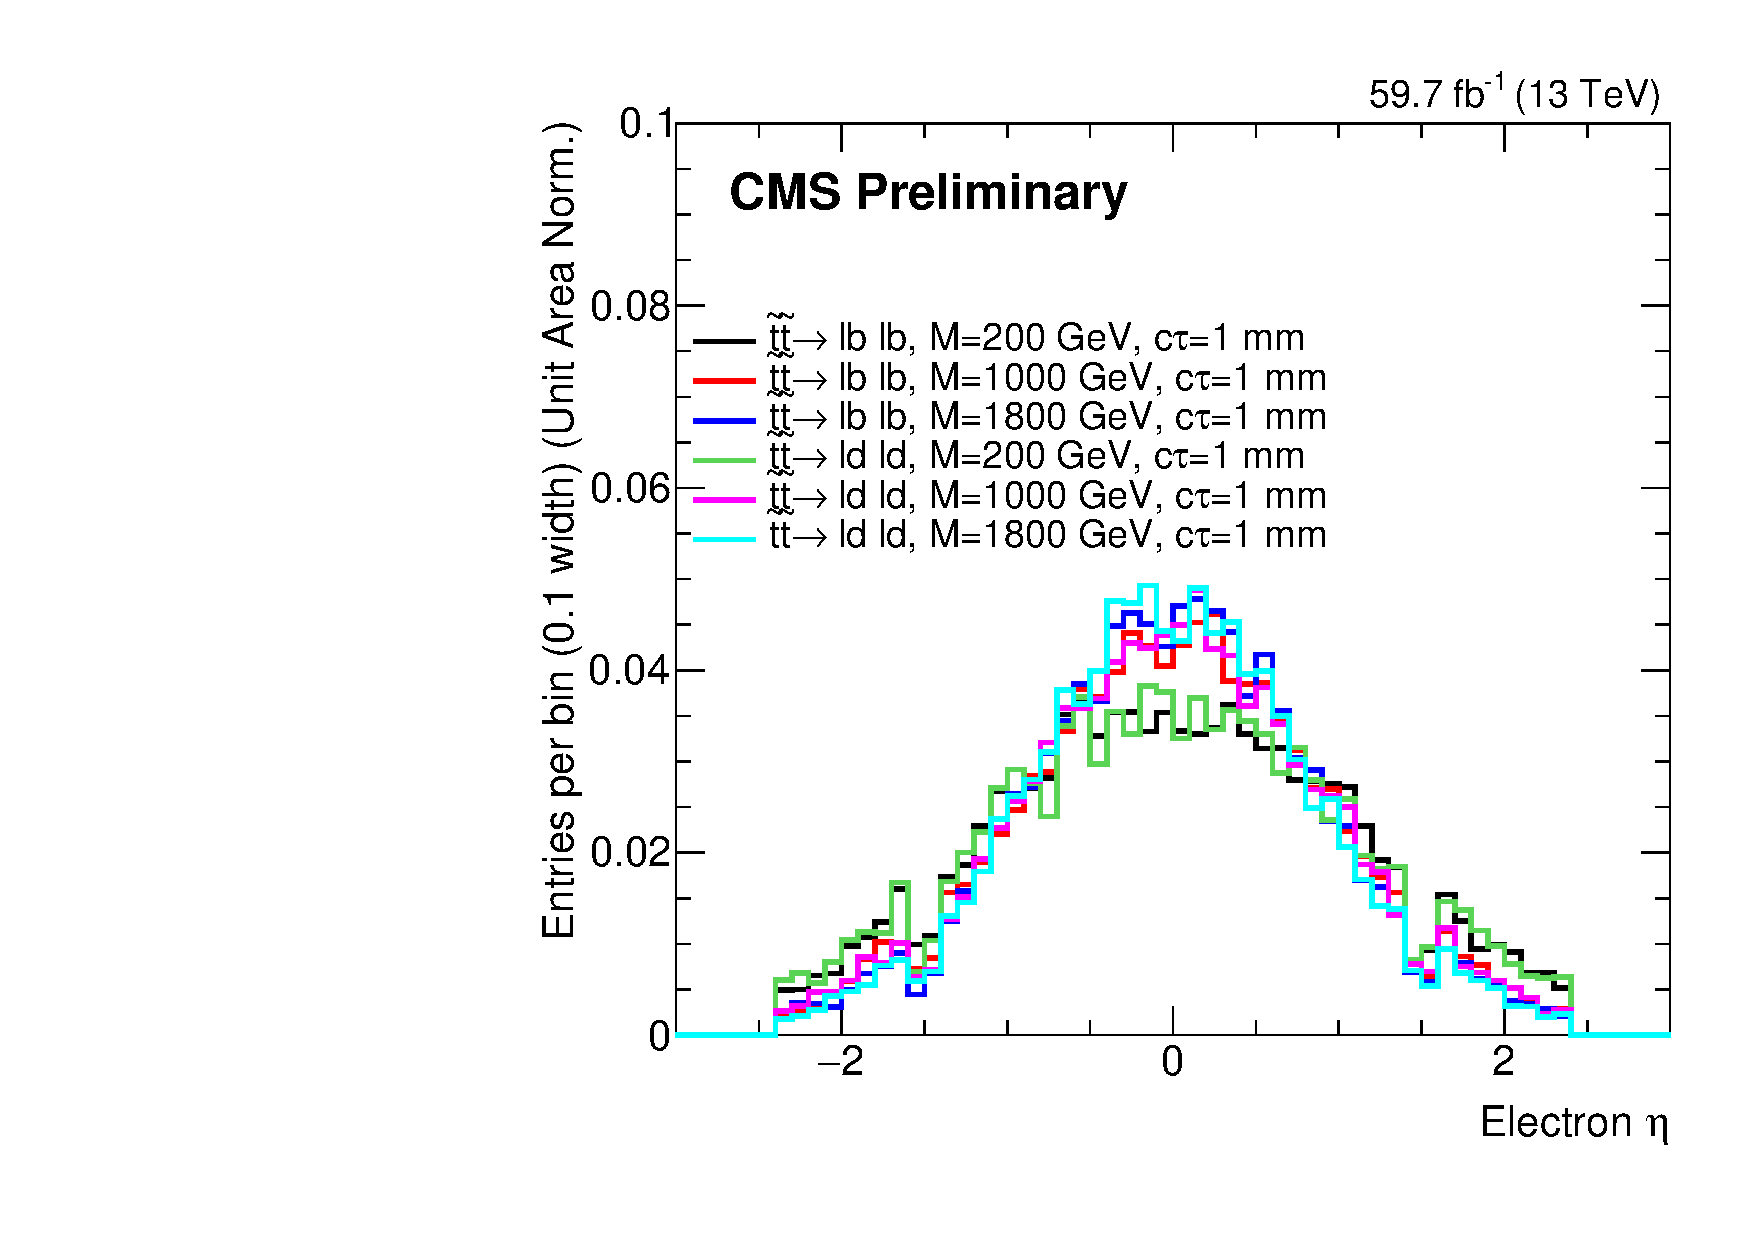
\includegraphics[width=0.45\textwidth]{figures/large_eta/electronEtaSignal.pdf}
\caption{Electron $\eta$ distribution for simulated background events in which the electron parent particles are required to be SM mesons (left). Electron $\eta$ distribution for simulated \stoptolb events (right). The $\Pe\Pgm$ preselection with a loosened $\eta$ requirement is applied in both plots.}
\label{large_eta_e}
\end{figure}

\pagebreak